\documentclass{article}
\usepackage[accepted]{icml2018}
\usepackage{graphicx}

\icmltitlerunning{Report Title}

\begin{document}

\twocolumn[
\icmltitle{E0:270 - Machine Learning - Neural Network Pruning Techniques}

\icmlsetsymbol{equal}{*}

\begin{icmlauthorlist}
\icmlauthor{Braunstein, Cameron}{dep2}
\icmlauthor{Nair, Abhishek}{dep1}
\icmlauthor{Shaw, Vishal}{dep1}
\end{icmlauthorlist}

\icmlaffiliation{dep1}{Department of Computer Science and Automation, Indian Institute of Science, Bangalore}
\icmlaffiliation{dep2}{Mathematics Department, Indian Institute of Science, Bangalore}

\icmlcorrespondingauthor{Braunstein, Cameron}{comeronb@iisc.ac.in}
\icmlcorrespondingauthor{Nair, Abhishek}{abhisheknair@iisc.ac.in}
\icmlcorrespondingauthor{Shaw, Vishal}{vishalshaw@iisc.ac.in}

\icmlkeywords{neural network, pruning, machine learning}

\vskip 0.3in
]

\printAffiliationsAndNotice{}

\begin{abstract}
This project investigated various methods of pruning a neural network. We have found that
The abstract should be ideally less than 10 short sentences. Among other things, provide information about what is your objective and how much progress has been made. 
\end{abstract}

\section{Introduction}
\label{introduction}
The PDF report should contain at most two pages excluding references and appendix and at most four pages including everything. Write about a subset of the following things that applies to your project:

\begin{enumerate}
	\item Problem Statement
	\item Motivation
	\item Literature Review
	\item Dataset description
	\item Preliminary Results
	\item Future Work
\end{enumerate}
\section{Literature Review}
\label{Literature Review}
The Optimal Brain Surgeon algorithm (OBS) as described by Hassibi, Stork and Wolff (put citation), prunes weights based on their calculated effect on the error using a second order Taylor expansion of the error function, and adjusts the unpruned weights to compensate. Layerwise OBS (L-OBS) as described by Dong, Chen and Pan simplifies the OBS algorithm by only considering a weight's effect on local error. They demonstrate that any increase in the global error from pruning a weight is reasonably bounded above by the corresponding increase in local error by pruning that weight. Because of this, L-OBS approximates OBS and is more computationally feasible.

\section{Model description}
\label{Model description} For our experiments, we trained a 748-300-100-10 feed foward neural network to classify the MNIST dataset. We then tested several pruning algorithms on the network. We implemented magnitude based weight pruning as a control. We ran a simplified version of the L-OBS algorithm, which recalculated the inverse Hessian only after every 2000 pruned weights. We also ran this simplified L-OBS algorithm, with a 3 titration retraining after every 2000 pruned weights and then a recalculation of the inverse Hessian. In the original L-OBS algorithm, the inverse Hessian is recalculated after every pruned weight. However this change was made out of computational necessity.

\section{Preliminary Results}
\label{Preliminary Results}

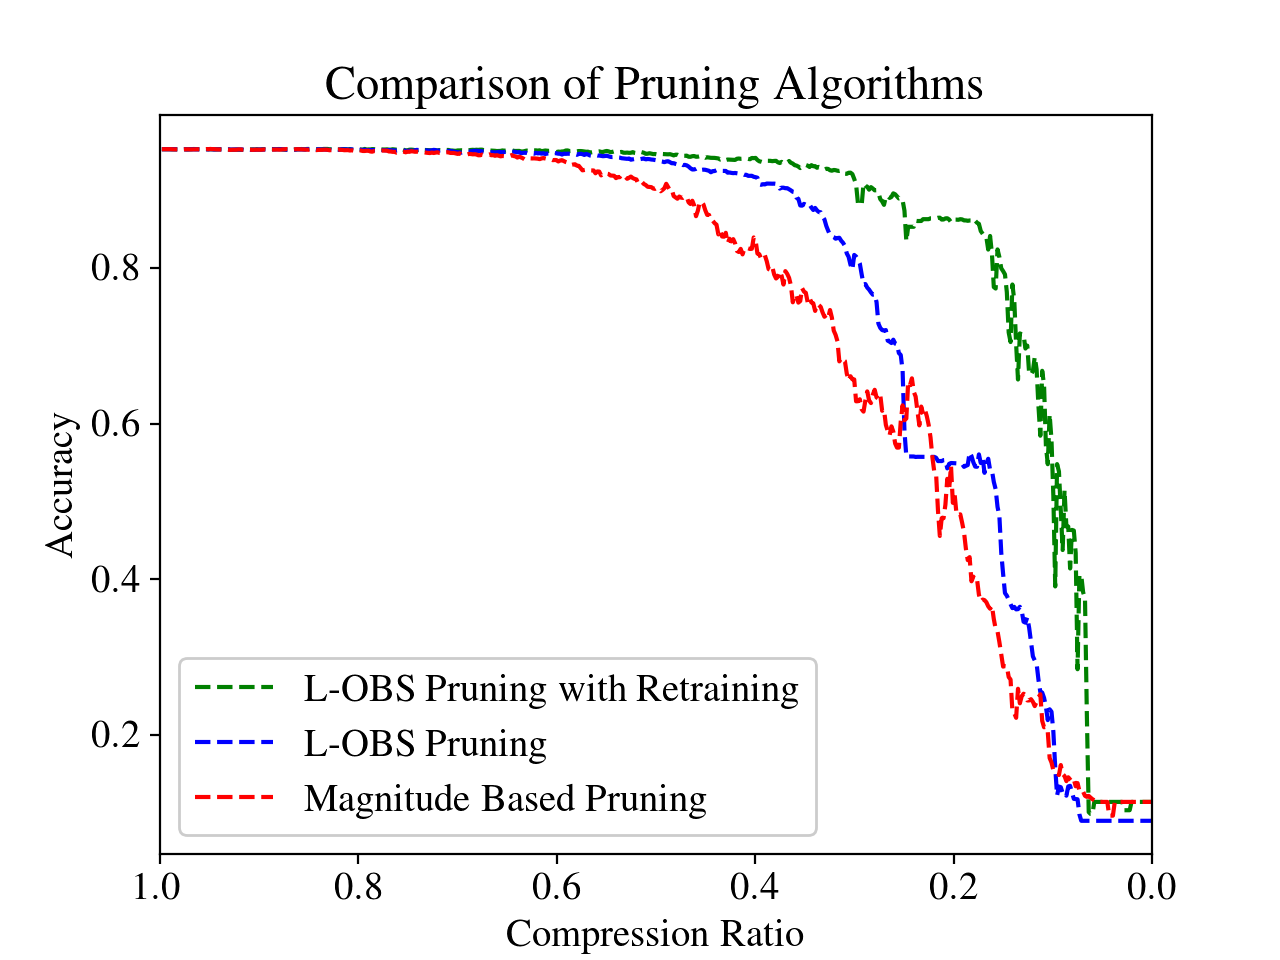
\includegraphics[scale=0.65]{Comparison}

Our control, the Magnitude Based Pruning, dropped in accuracy the fastest, followed by our simplified L-OBS algorithm and then simplified L-OBS with retraining. The L-OBS with retraining graph is particularly jagged, as retraining every 2000 prunings resulted in spikes of accuracy, particularly as the network became more sparse. Interestingly, all algorithms stayed closed to their initial test accuracy until a compression ratio of approximately 0.6. This suggests that the network has redundancies which can be eliminated before training begins.

\section{Future Work}
\label{Future Work}

We hope to combine several of our tested algorithms to see if we can achieve even better compression without loss in accuracy.

You can additionally provide anything else that is relevant to your project but is not present in the list given above. 

You can create various sections/subsections etc. to organize your report as per the need. Use \texttt{biblio.bib} file to provide references. The references should be provided by using cite keyword \cite{langley00}.

You can contact your project mentor if you have any confusion.


%%%%%%%%%%%%%%%%%%%%%%%%%%%%%%%%%%%%%%%%%%%%%%%%%%%%%%%%%%%%%%%%%%%%%%%%%%%%%%%
\newpage

\bibliography{biblio}
\bibliographystyle{icml2018}


%%%%%%%%%%%%%%%%%%%%%%%%%%%%%%%%%%%%%%%%%%%%%%%%%%%%%%%%%%%%%%%%%%%%%%%%%%%%%%%
% Remove this part if you are not using an Appendix. Appendix is ungraded. The
% reader may wish to ignore the appendix altogether. Write everything that you
% think is important in the main report text only.

\appendix
\section{Optional Appendix (Ungraded)}
Remove this part if you are not using an Appendix. Appendix is ungraded. The
reader may wish to ignore the appendix altogether. Write everything that you
think is important in the main report text only.

%%%%%%%%%%%%%%%%%%%%%%%%%%%%%%%%%%%%%%%%%%%%%%%%%%%%%%%%%%%%%%%%%%%%%%%%%%%%%%%

\end{document}